%%%%%%%%%%%%%%%%%%%%%%%%%%%%%%%%%%%%%%%%%
% Stylish Article
% LaTeX Template
% Version 2.1 (1/10/15)
%
% This template has been downloaded from:
% http://www.LaTeXTemplates.com
%
% Original author:
% Mathias Legrand (legrand.mathias@gmail.com) 
% With extensive modifications by:
% Vel (vel@latextemplates.com)
%
% License:
% CC BY-NC-SA 3.0 (http://creativecommons.org/licenses/by-nc-sa/3.0/)
%
%%%%%%%%%%%%%%%%%%%%%%%%%%%%%%%%%%%%%%%%%

%----------------------------------------------------------------------------------------
%	PACKAGES AND OTHER DOCUMENT CONFIGURATIONS
%----------------------------------------------------------------------------------------

\documentclass[fleqn,10pt]{SelfArx} % Document font size and equations flushed left

\usepackage[english]{babel} % Specify a different language here - english by default

\usepackage{lipsum} % Required to insert dummy text. To be removed otherwise

\captionsetup[figure]{justification=justified, singlelinecheck=off} 
\captionsetup[table]{justification=justified, singlelinecheck=off} 

%----------------------------------------------------------------------------------------
%	COLUMNS
%----------------------------------------------------------------------------------------

\setlength{\columnsep}{0.55cm} % Distance between the two columns of text
\setlength{\fboxrule}{0.75pt} % Width of the border around the abstract
\linespread{1.5}

%----------------------------------------------------------------------------------------
%	COLORS
%----------------------------------------------------------------------------------------

\definecolor{color1}{RGB}{0,0,90} % Color of the article title and sections
\definecolor{color2}{RGB}{10,20,20} % Color of the boxes behind the abstract and headings
\definecolor{xsubj}{RGB}{243,194,68} 
\definecolor{xsess}{RGB}{53,99,161} 
\definecolor{xsamp}{RGB}{18,165,121} 

%----------------------------------------------------------------------------------------
%	HYPERLINKS
%----------------------------------------------------------------------------------------

\usepackage{hyperref} % Required for hyperlinks
\hypersetup{hidelinks,colorlinks,breaklinks=true,urlcolor=color2,citecolor=color1,linkcolor=color1,bookmarksopen=false,pdftitle={Title},pdfauthor={Author}}
%----------------------------------------------------------------------------------------
%	ARTICLE INFORMATION
%----------------------------------------------------------------------------------------

% \JournalInfo{Journal, Vol. XXI, No. 1, 1-5, 2013} % Journal information
\JournalInfo{$ $ } % Journal information
\Archive{Pre-print} % Additional notes (e.g. copyright, DOI, review/research article)

\PaperTitle{\new{Induced} Numerical Instabilities in Analytical Pipelines Lead to \new{Impactful} Variability in Brain Networks} % Article title

\Authors{Gregory Kiar\textsuperscript{1}, Yohan Chatelain\textsuperscript{2}, Pablo de Oliveira Castro\textsuperscript{3},
Eric Petit\textsuperscript{4}, Ariel Rokem\textsuperscript{5}, Gaël Varoquaux\textsuperscript{6},
Bratislav Misic\textsuperscript{1}, Alan C. Evans\textsuperscript{1$\dagger$}, Tristan Glatard\textsuperscript{2$\dagger$}} % Authors
\affiliation{\textsuperscript{1}\textit{Montréal Neurological Institute, McGill University, Montréal, QC, Canada}}
\affiliation{\textsuperscript{2}\textit{Department of Computer Science and Software Engineering, Concordia University, Montréal, QC, Canada}}
\affiliation{\textsuperscript{3}\textit{Department of Computer Science, Université of Versailles, Versailles, France}}
\affiliation{\textsuperscript{4}\textit{Exascale Computing Lab, Intel, Paris, France}}
\affiliation{\textsuperscript{5}\textit{Department of Psychology and eScience Institute, University of Washington, Seattle, WA, USA}}
\affiliation{\textsuperscript{6}\textit{Parietal project-team, INRIA Saclay-ile de France, France}}
\affiliation{$\dagger$Authors contributed equally}

\Keywords{Stability --- Reproducibility --- Network Neuroscience --- Neuroimaging} % Keywords - if you don't want any simply remove all the text between the curly brackets
\newcommand{\keywordname}{Keywords} % Defines the keywords heading name

%----------------------------------------------------------------------------------------
%	ABSTRACT
%----------------------------------------------------------------------------------------

\Abstract{The analysis of brain-imaging data requires complex processing pipelines to support findings on brain
function or pathologies. Recent work has shown that variability in analytical decisions, \new{small amounts of noise,
or computational environments} can lead to substantial
differences in the results, endangering the trust in
conclusions~\cite{botvinik2020variability,bennett2009neural,eklund2016cluster,Kiar2020-lb,salari2020file,Lewis2017-ll,Glatard2015-vc}.
We explored the instability of results by instrumenting a connectome estimation pipeline with Monte Carlo
Arithmetic~\cite{Parker1997-qq,Denis2016-wo} to introduce random noise throughout. We evaluated the reliability of the
connectomes, their features~\cite{Betzel2018-eo,Rubinov2010-fh}, and the impact on
analysis~\cite{Park2015-uj,Gupta2015-ap}. The stability of results was found to range from perfectly stable to highly
unstable. This paper highlights the potential of leveraging induced variance in estimates of brain connectivity to
reduce the bias in networks alongside increasing the robustness of their applications in the classification of
individual differences. We demonstrate that stability evaluations are necessary for understanding error inherent to
\new{brain imaging experiments}, and how numerical analysis can be applied to typical analytical workflows \new{both in brain
imaging and other domains of computational science}. Overall, while the
extreme variability in results due to analytical instabilities could severely hamper our understanding of brain
organization, it also leads to an increase in the reliability of datasets.}

%----------------------------------------------------------------------------------------

\newcommand{\new}[1]{{\color{blue} #1}}

\begin{document}

\flushbottom % Makes all text pages the same height
\maketitle % Print the title and abstract box
% \tableofcontents % Print the contents section
\thispagestyle{empty} % Removes page numbering from the first page

%----------------------------------------------------------------------------------------
%	ARTICLE CONTENTS
%----------------------------------------------------------------------------------------

The modelling of brain networks, called connectomics, has shaped our understanding of the structure and function
of the brain across a variety of organisms and scales over the last
decade~\cite{behrens2012human,xia2016connectomic,morgan2013not,van2016comparative,Rubinov2010-fh,Dubois2016-yr}.
In humans, these wiring diagrams are obtained \textit{in vivo} through Magnetic Resonance Imaging (MRI), and show
promise towards identifying biomarkers of disease. This can not only improve understanding of so-called
``connectopathies'', such as Alzheimer's Disease and Schizophrenia, but potentially pave the way for
therapeutics~\cite{fornito2015connectomics,deco2014great,xie2012mapping,filippi2013assessment,van2014brain}.

However, the analysis of brain imaging data relies on complex computational methods and software. Tools are
trusted to perform everything from pre-processing tasks to downstream statistical evaluation. While these tools
undoubtedly undergo rigorous evaluation on bespoke datasets, in the absence of ground-truth this is often evaluated
through measures of reliability~\cite{Bartko1966-tl,Brandmaier2018-tk,bridgeford2020elim,Kiar2018-jt}, proxy outcome
statistics, or agreement with existing theory. Importantly, this means that tools are not necessarily of known or
consistent quality, and it is not uncommon that equivalent experiments may lead to diverging
conclusions~\cite{botvinik2020variability,Lewis2017-ll,Glatard2015-vc,salari2020file}. While many scientific
disciplines suffer from a lack of reproducibility~\cite{baker20161}, this was recently explored in brain imaging by a
$70$ team consortium which performed equivalent analyses and found widely inconsistent
results~\cite{botvinik2020variability}, and it is likely that software instabilities played a role.

The present study approached evaluating reproducibility from a computational perspective in which a series of brain
imaging studies were numerically perturbed \new{in} such \new{a way} that the plausibility of results was not affected, and the
implications of the observed instabilities \new{on downstream analyses} were quantified. We accomplished this through the use of Monte Carlo
Arithmetic (MCA)~\cite{Parker1997-qq}, a technique which enables characterization of the sensitivity of a system to
small \new{numerical} perturbations. \new{This is importantly distinct from data perturbation experiments where the underlying
datasets are manipulated or pathologies may be simulated, and allows for the evaluation of experimental uncertainty in real-world
settings.} We explored the impact of \new{numerical} perturbations through the direct comparision of structural connectomes,
the consistency of their features, and their eventual application in a neuroscience study. \new{We also characterized the}
consequences \new{of instability in these pipelines on the reliability of derived datasets,} and \new{discuss how the induced
variability may be harnessed to increase the discriminability of datasets}. \new{Finally, we} make recommendations for
the roles \new{perturbation} analyses may play in brain imaging research \new{and beyond}.

%------------------------------------------------
\subsection*{Graphs Vary Widely With Perturbations}
\begin{figure*}[hbt]\centering
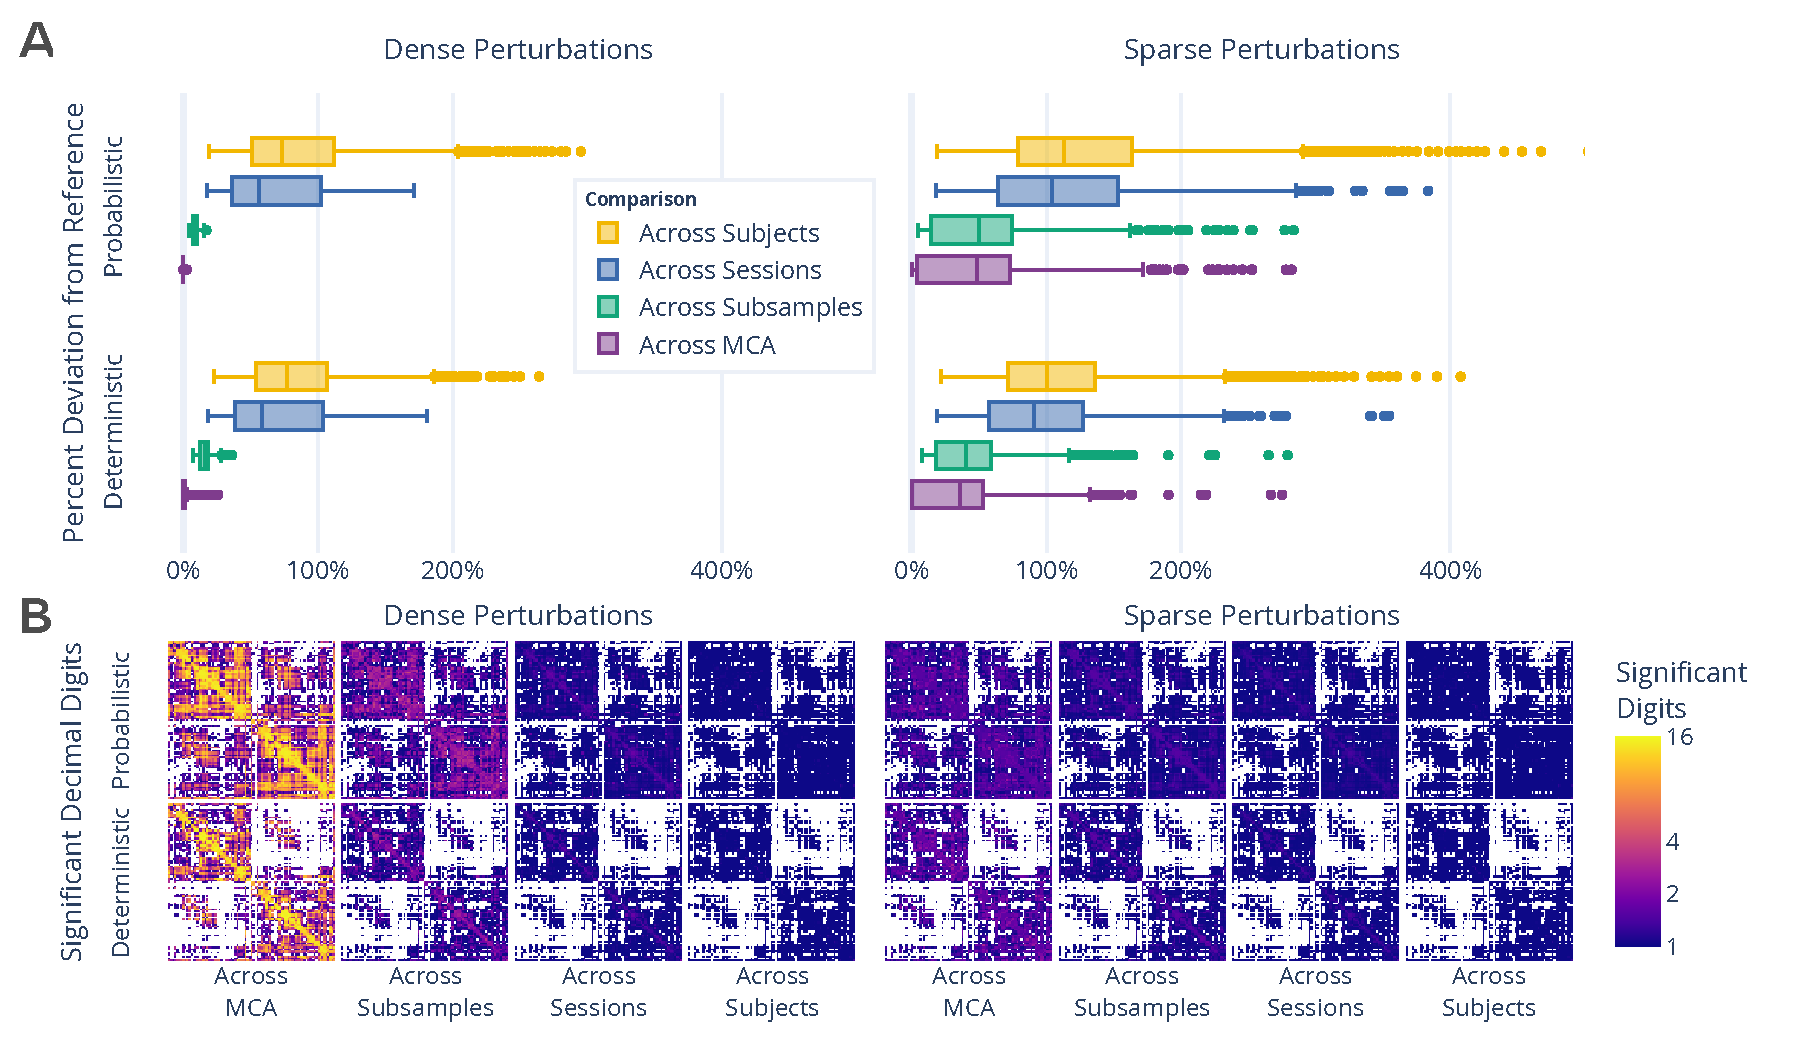
\includegraphics[width=0.98\linewidth]{figures/fig1_absolute_differences.pdf}
\caption{Exploration of perturbation-induced deviations from reference connectomes.
(\textbf{A}) The absolute deviations, in the form of normalized percent deviation from reference, shown as the
across MCA series relative to Across Subsample, Across Session, and Across Subject variations.
(\textbf{B}) The number of significant decimal digits in each set of connectomes as obtained after evaluating the
effect of perturbations. In the case of 16, values can be fully relied upon, whereas in the case of 1 only the first
digit of a value can be trusted. \new{Dense} and \new{sparse} perturbations are shown on the left and right, respectively.}
\label{fig:absolute}
\end{figure*}

Prior to exploring the analytic impact of instabilities, a direct understanding of the induced variability was
required. A subset of the Nathan Kline Institute Rockland Sample (NKIRS) dataset~\cite{Nooner2012-eg} was randomly
selected to contain $25$ individuals with two sessions of imaging data, each of which was subsampled into two
components, resulting in four \new{samples} per individual \new{and $100$ samples total ($25 \times 2 \times 2$ samples)}. Structural connectomes were generated with canonical
deterministic and probabilistic pipelines~\cite{Garyfallidis2014-ql,Garyfallidis2012-gg} which were instrumented with
MCA, replicating computational noise either \new{sparsely} or \new{densely} throughout the pipelines~\cite{Denis2016-wo,Kiar2020-lb}.
\new{In the sparse case, a small subset of the libraries were instrumented with MCA, allowing for the evaluation of the
cascading effects of numerical instabilities that may arise. In the dense case, operations are more uniformly perturbed
and thus the law of large numbers suggests that perturbations will quickly offset one-another and only dramatic local
instabilities will have propagating effects. Importantly, the perturbations resulting from the sparse setting
represent a strict subset of the possible outcomes of the dense implementation. The random perturbations are statistically independent from one another
across both settings and simulations. Instrumenting pipelines with MCA increases their computation time, in this
case by multiplication factors of $1.2 \times$ and $7 \times$ for the sparse and dense settings, respectively~\cite{Kiar2020-lb}.
The results obtained were compared to unperturbed (e.g. reference) connectomes in both cases.}
The \new{connectomes} were sampled \new{$10$} times per \new{sample} and once without perturbations, resulting in a total of
$4,200$ connectomes. \new{Two versions of the unperturbed connectomes were generated and compared such that the absence
of variability aside from that induced via MCA could be confirmed}.

The stability of connectomes was evaluated through the \new{normalized percent} deviation from reference~\cite{Kiar2020-lb} and the number
of significant digits
(Figure~\ref{fig:absolute}). The comparisons were grouped according to differences across simulations, subsampling
of data, sessions of acquisition, or subjects, \new{and accordingly sorted from most to least similar}. While the
similarity of connectomes decreases as the collections become
more distinct, connectomes generated with input perturbations show considerable variability, often reaching deviations
equal to or greater than those observed across individuals or sessions (Figure~\ref{fig:absolute}A; right).
\new{Interpretting these results with respect to the distinct MCA environments used suggests that the tested pipelines
may not suffer from single dominant sources of instability, but that nevertheless there exist minor local instabilities
which may the propagate throughout the pipeline. Furthermore,} this
finding suggests that instabilities inherent to these pipelines may mask session or individual differences, limiting
the trustworthiness of derived connectomes. While both pipelines show similar performance, the probabilistic pipeline
was more stable in the face of pipeline perturbations whereas the deterministic was more stable to input perturbations
($p < 0.0001$ for all; exploratory). \new{As an alternative to the normalized percent deviation, the stability of}
correlations \new{between} networks can be found in \sref{supsec:correlation}.

The number of significant digits per edge across connectomes (Figure~\ref{fig:absolute}B) similarly decreases
\new{alongside the decreasing similarity between comparison groups}. While the cross-MCA comparison of connectomes generated with pipeline perturbations show nearly perfect
precision for many edges (approaching the maximum of $15.7$ digits for $64$-bit data), this evaluation uniquely shows
considerable drop off in performance \new{when comparing networks across} subsamplings (average of $< 4$ digits). In addition, \new{sparsely
perturbed connectomes} show no more than an average of $3$ significant digits across all \new{comparison} groups, demonstrating a significant
limitation in the reliability \new{of} independent edge weights. \new{The number of significant digits} across individuals did not exceed a single digit
per edge in any case, indicating that only the order \new{of} magnitude of edges in naively computed groupwise average connectomes can
be trusted. The combination of these results with those presented in Figure~\ref{fig:absolute}A suggests that while
specific edge weights are largely affected by instabilities, macro-scale network \new{organization} is stable.

\subsection*{\new{Perturbations Increase Biologically-Driven Discriminability}}
\begin{table*}[ht]\centering
\caption{The impact of instabilities as evaluated through the \new{discriminability} of the dataset based on individual (or
subject) differences, session, and subsample. The performance is reported as mean discriminability. While a perfectly
\new{discriminable} dataset would be represented by a score of $1.0$, the chance performance, indicating minimal \new{discriminability}, is
$1 /$the number of classes. $H_3$ could not be tested using the reference executions due to too few possible
comparisons. The alternative hypothesis, indicating significant \new{discrimination}, was accepted for all experiments, with
$p < 0.005$.}
\vspace{5pt}
% \fcolorbox{color1}{white}{%
% \parbox{\textwidth-2\fboxsep-2\fboxrule}{\centering
%   \colorbox{color2!10}{
%     \parbox{\textwidth-4\fboxsep-2\fboxrule}{

\begin{tabular}{lllcccc}
 \cellcolor{color1!10}          & \cellcolor{color1!10}   &  \cellcolor{color1!10} & \cellcolor{color1!10} \textbf{Unscaled Ref.} & \cellcolor{color1!10} \textbf{Scaled Ref.} & \cellcolor{color1!10}\textbf{Dense MCA} & \cellcolor{color1!10} \textbf{Sparse MCA} \\
\cellcolor{color1!10}\textbf{Comparison} & \cellcolor{color1!10}\textbf{Chance} & \cellcolor{color1!10}\textbf{Target} & \cellcolor{color1!10}Det. \quad Prob. & \cellcolor{color1!10}Det. \quad Prob. & \cellcolor{color1!10} Det. \quad Prob. & \cellcolor{color1!10}Det. \quad Prob. \\
\hline
$H_{1}$: Across Subjects  & $0.04$& $1.0$& $0.64$\quad$0.65$ &$0.82$\quad$0.82$& $0.82$\quad$0.82$& $0.77$\quad$0.75$\\
$H_{2}$: Across Sessions  & $0.5$ & $0.5$& $1.00$\quad$1.00$ &$1.00$\quad$1.00$& $1.00$\quad$1.00$& $0.88$\quad$0.85$\\
$H_{3}$: Across Subsamples& $0.5$ & $0.5$&                   &                 & $0.99$\quad$1.00$& $0.71$\quad$0.61$\\
\end{tabular}

%     }
%   }
% }%
% }%

\label{tab:discrim}
\end{table*}

We assessed the reproducibility of the dataset through mimicking and extending a typical test-retest
experiment~\cite{bridgeford2020elim} in which the similarity of samples across \new{sessions} were
compared to distinct samples in the dataset (Table~\ref{tab:discrim}, with additional experiments and explanation in
\sref{supsec:discrimfull}). The ability to \new{discriminate} connectomes across subjects (Hypothesis~1) is an essential
prerequisite for the application of brain imaging towards identifying individual differences~\cite{Dubois2016-yr}. In
testing hypothesis~1, we observe that the dataset is \new{discriminable} with a score of $0.64$ and $0.65$ ($p < 0.001$; optimal
score: $1.0$; chance: $0.04$) \new{for the Deterministic and Probabilistic pipelines, respectively, in the absence of MCA}.
However, we can see that inducing instabilities through MCA improves the \new{discriminability} of the dataset to over
$0.75$ in each case ($p < 0.001$ for all), significantly higher than without instrumentation ($p < 0.005$ for all).
\new{The definition of the discriminability statistic is such that if all samples derived from the a given session were
near replicates of one another the score would be unchanging despite the increased sample size~\cite{bridgeford2020elim}}.
Th\new{e} result\new{ing increase in discriminability} therefore suggests the utility of perturbation methods for
synthesizing robust and reliable individual estimates of connectivity, serving as a cost effective and context-agnostic
method for dataset augmentation.

While the \new{discriminability} of individuals is essential for the identification of \new{individual} brain networks,
it is similarly reliant on
network similarity \new{– or lack of discriminability –} across equivalent acquisitions (Hypothesis~2). In this case,
connectomes were grouped based upon session, rather than subject, and the ability to distinguish one session from
another \new{based on subsamples} was computed within-individual and aggregated. Both the unperturbed and \new{dense}
perturbation settings perfectly preserved differences between sessions with a score of $1.0$ ($p < 0.005$; optimal
score: $0.5$; chance: $0.5$), indicating a dominant session-dependent signal for all individuals despite no intended
biological differences. However, while still significant relative to chance (score: $0.85$ and $0.88$; $p < 0.005$ for
both), \new{sparse} perturbations lead to significantly lower discriminability of the dataset ($p < 0.005$ for all).
This reduction of the difference between sessions suggests that \new{the added} variance \new{due to} perturbations
reduces the \new{relative} impact of non-biological acquisition-dependent bias inherent in the \new{networks}.

Though the previous sets of experiments inextricably evaluate the interaction between \new{data acquisition} and tool,
the use of subsampling allowed for characterizing the discriminability of networks sampled from within a single
acquisition (Hypothesis~3). While this experiment could not be evaluated using reference executions, the \new{networks
generated with dense} perturbations showed near perfect discrimination between subsamples, with scores of $0.99$ and
$1.0$ ($p < 0.005$; optimal: $0.5$; chance: $0.5$). Given that there is no variability in data acquisition\new{, due to
undesired effects such as participant motion,} or preprocessing, the \new{ability to discriminate between equivalent
subsamples} in this experiment may only be due to instability or bias inherent to the pipelines. The high variability
introduced through \new{sparse} perturbations considerably lowered the \new{discriminability} towards chance (score:
$0.71$ and $0.61$; $p < 0.005$ for all), further supporting this as an effective method for obtaining lower-bias
estimates of individual connectivity.

Across all cases, the induced perturbations \new{led to an increased ability to discriminate networks on the basis} of
meaningful biological signal alongside a reduction \new{in discriminability due to} of off-target signal. This result
appears strikingly like a manifestation of the well-known bias-variance
tradeoff~\cite{geman1992neural} in machine learning, a concept which observes a decrease in bias as variance is
favoured by a model. In particular, this highlights that numerical perturbations can be used to not only evaluate the
stability of pipelines, but that the induced variance may be leveraged for the interpretation as a robust distribution
of possible results.

\subsection*{Distributions of Graph Statistics \new{Were} Reliable, But Individual Statistics \new{Were} Not}
\begin{figure*}[bht!]\centering
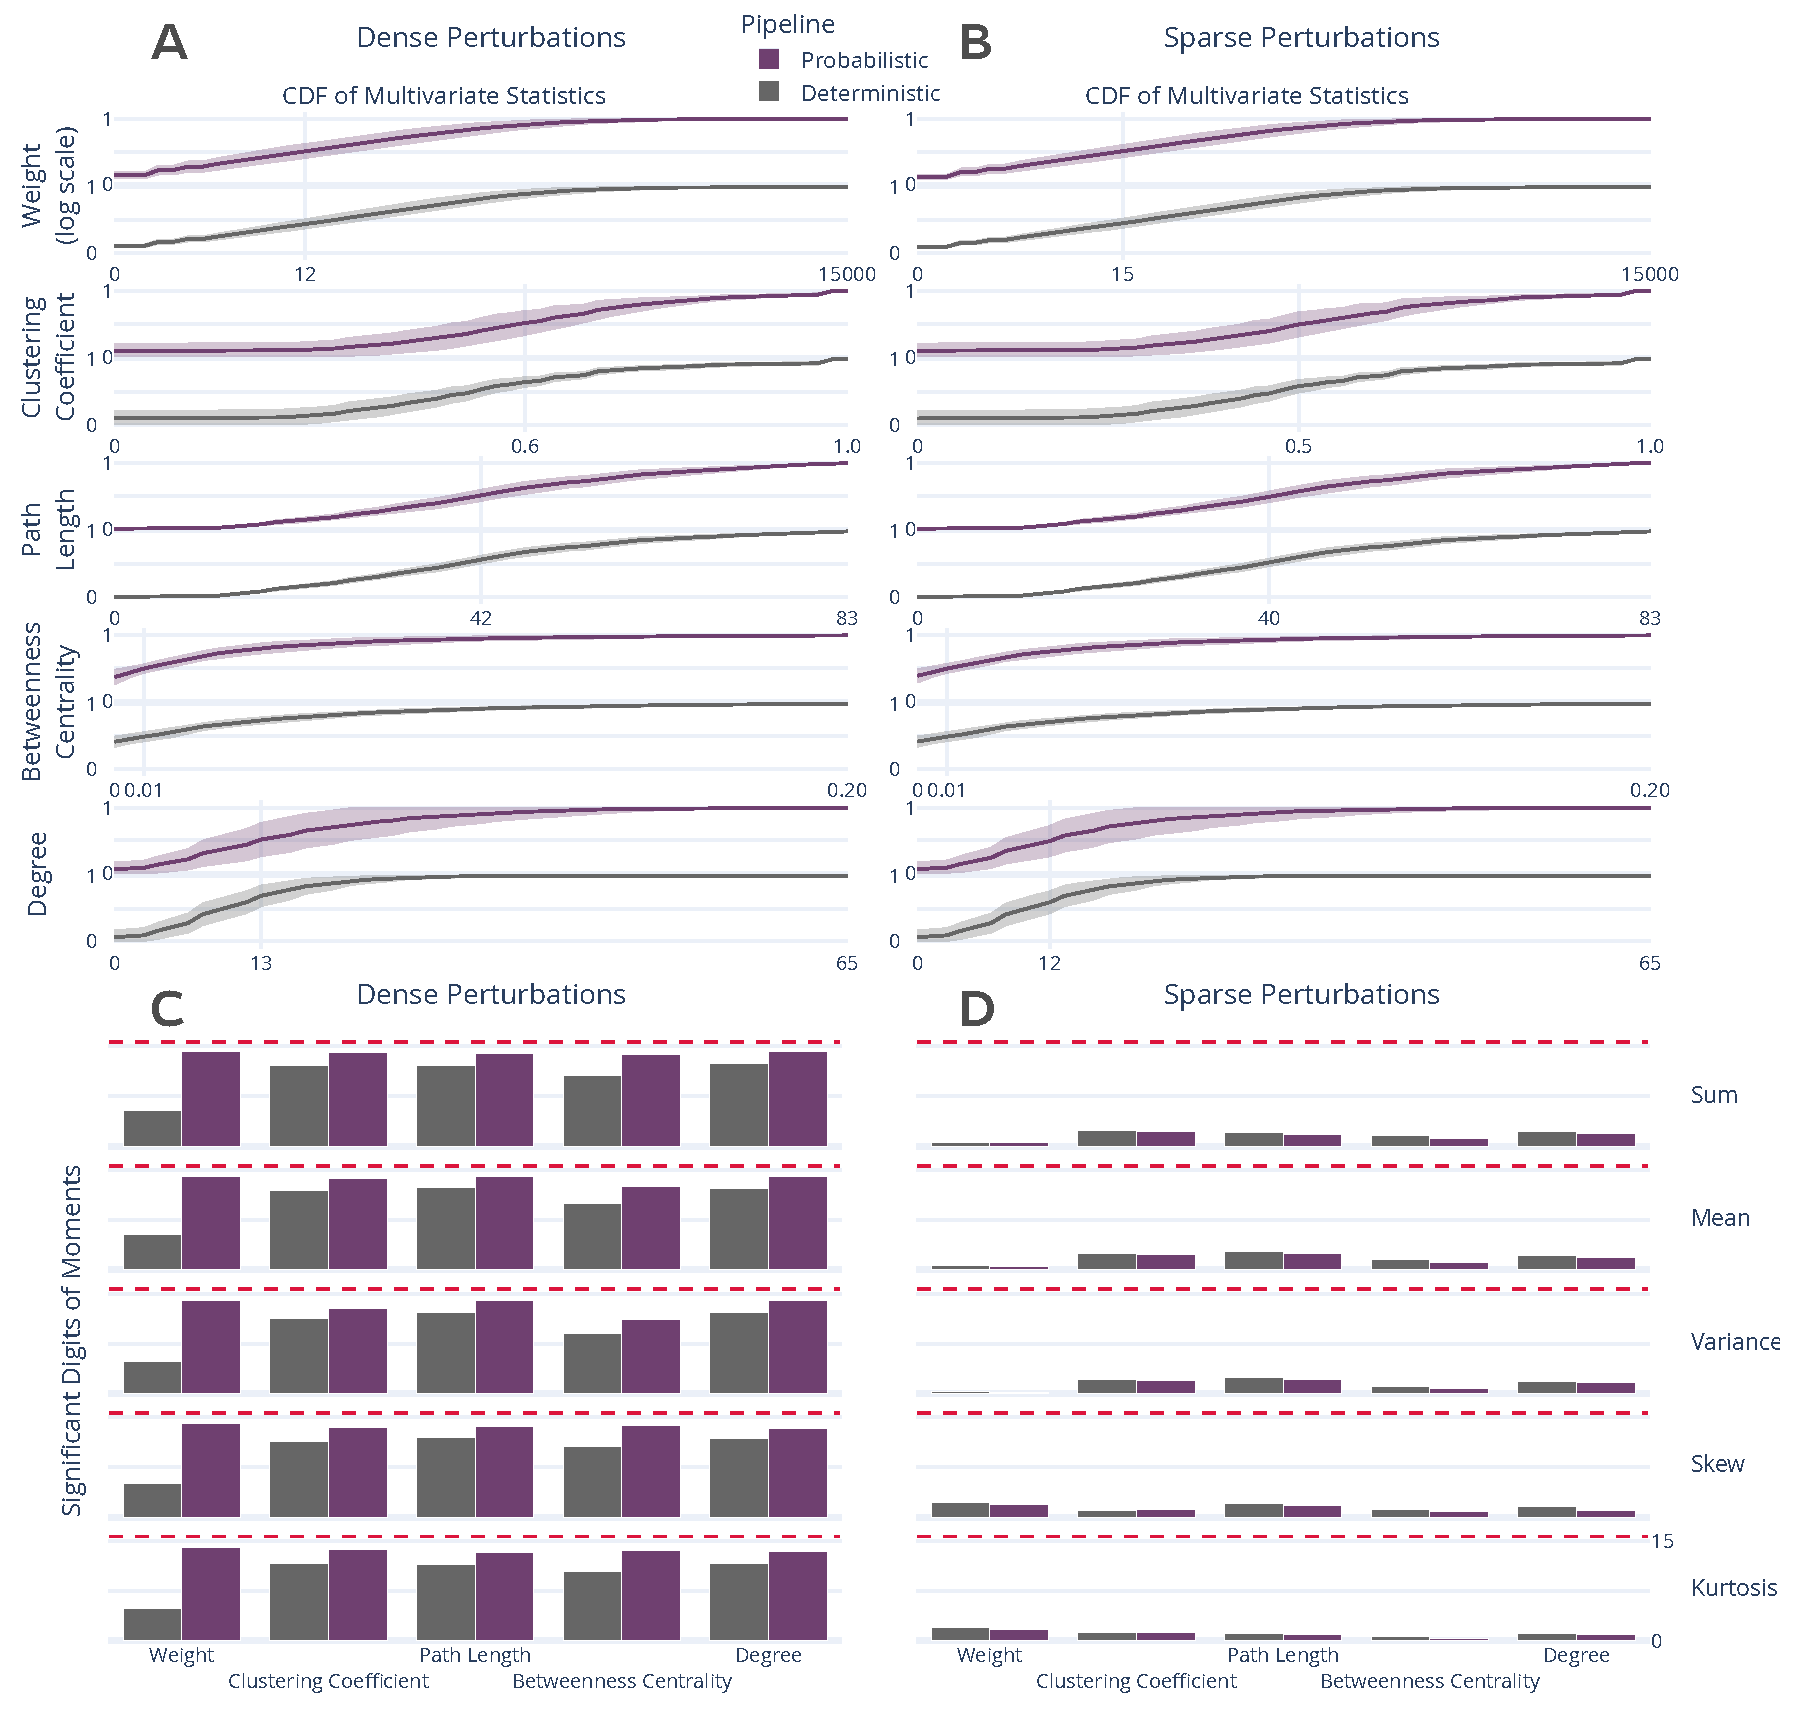
\includegraphics[width=\linewidth]{figures/fig2_multivariate_differences.pdf}
\caption{Distribution and stability assessment of multivariate graph statistics. (\textbf{A}, \textbf{B}) The
cumulative distribution functions of multivariate statistics across all subjects and perturbation settings. There was
no significant difference between the distributions in A and B. (\textbf{C}, \textbf{D}) The number of significant
digits in the first $5$ five moments of each statistic across perturbations. The dashed red line refers to the maximum
possible number of significant digits.}
\label{fig:multivar}
\end{figure*}

Exploring the stability of topological features of connectomes is relevant for typical analyses, as low dimensional
features are often more suitable than full connectomes for many analytical methods in practice~\cite{Rubinov2010-fh}.
A separate subset of the NKIRS dataset was randomly selected to contain a single non-subsampled session for $100$
individuals \new{($100 \times 1 \times 1$) using the pipelines and instrumentation methods to generate connectomes as
above. Connectomes were generated $20$ times each, resulting in a dataset which also contained $4,200$ connectomes with
the MCA simulations serving as the only source of repeated measurements.}

The stability of several commonly-used multivariate graph features~\cite{Betzel2018-eo} \new{were} explored \new{and
are presented} in Figure~\ref{fig:multivar}. The cumulative density of the features was computed within individuals and
the mean \new{cumulative} density and associated standard error were computed for across individuals
(Figures~\ref{fig:multivar}A and \ref{fig:multivar}B). There was no significant difference between the distributions
for each feature across the two perturbation settings, suggesting that the topological features summarized by these
multivariate features are robust across both perturbation modes.

In addition to the comparison of distributions, the stability of the first $5$ moments of these features was evaluated
(Figures~\ref{fig:multivar}C and \ref{fig:multivar}D). In the face of \new{dense} perturbations, the feature-moments
were stable with more than $10$ significant digits with the exception of edge weight when using the deterministic
pipeline, though the probabilistic pipeline was more stable for all comparisons ($p < 0.0001$; exploratory). In stark
contrast, \new{sparse} perturbations led to highly unstable feature-moments (Figure~\ref{fig:multivar}D), such that
none contained more than $5$ significant digits of information and several contained less than a single significant
digit, indicating a complete lack of reliability. This dramatic degradation in stability for individual measures
strongly suggests that these features may be unreliable as individual biomarkers when derived from a single pipeline
evaluation, though their reliability may be increased when studying their distributions across perturbations. A similar
analysis was performed for univariate statistics \new{which obtained similar findings} and can be found in
\sref{supsec:univar}.

\subsection*{Uncertainty in Brain-Phenotype Relationships}

\begin{figure*}[ht]\centering
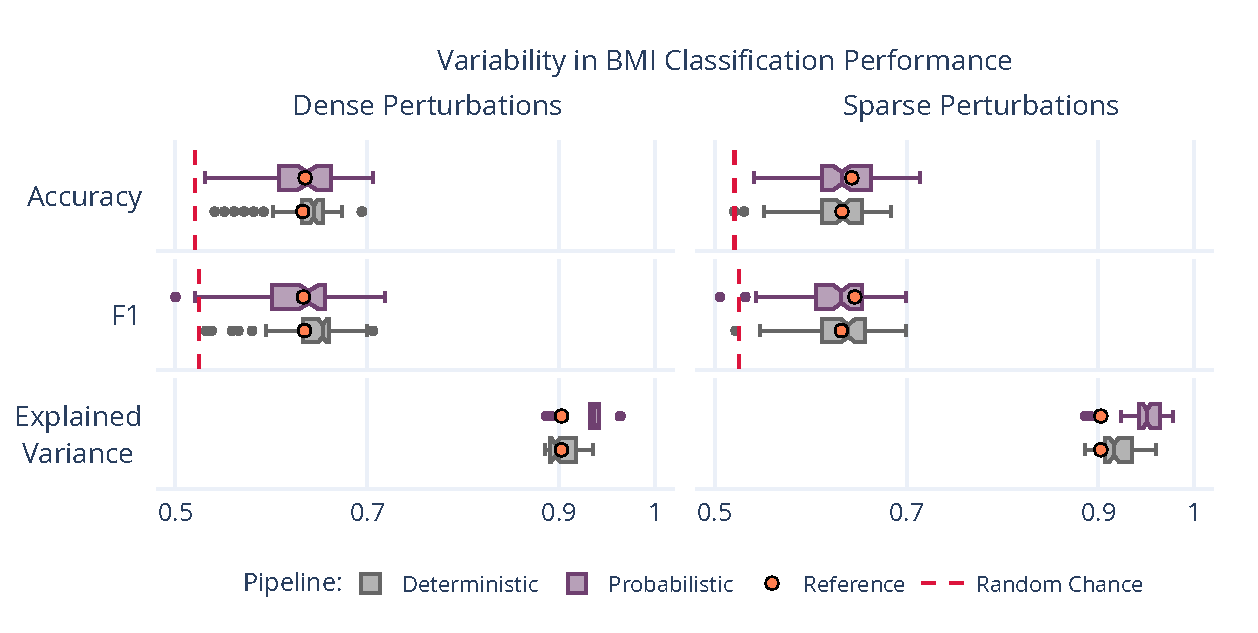
\includegraphics[width=0.7\linewidth]{figures/fig3_bmi_classification.pdf}
\caption{Variability in BMI classification across the sampling of an MCA-perturbed dataset. The dashed red lines
indicate random-chance performance, and the orange dots show the performance using the reference executions.}
\label{fig:bmi}
\end{figure*}
 
While the variability of connectomes and their features was summarized above, networks are commonly used as inputs to
machine learning models tasked with learning brain-phenotype relationships~\cite{Dubois2016-yr}. To explore the
stability of these analyses, we modelled the relationship between high- or low- Body Mass Index (BMI) groups and brain
connectivity using standard dimensionality reduction and classification tools~\cite{Park2015-uj,Gupta2015-ap}, and
compared this to reference and random performance (Figure~\ref{fig:bmi}).

The analysis was perturbed through distinct samplings of the dataset across both pipelines and perturbation methods.
The accuracy and F1 score for the perturbed models varied from $0.520$~–~$0.716$ and $0.510$~–~$0.725$, respectively,
ranging from at or below random performance to outperforming performance on the reference dataset. This large
variability illustrates a previously uncharacterized margin of uncertainty in the modelling of this relationship, and
limits confidence in reported accuracy scores on singly processed datasets. The portion of explained variance in these
samples ranged from $88.6\%$~-–~$97.8\%$, similar to the reference \new{of $90.3\%$}, suggesting that the range in
performance was not due to a gain or loss of meaningful signal, but rather the reduction of bias towards specific
outcome. Importantly, this finding does not suggest that modelling brain-phenotype relationships is not possible, but
rather it sheds light on impactful uncertainty that must be accounted for in this process, and supports the use of
ensemble modeling techniques.

\new{One distinction between the results presented here and the previous is that while networks derived from dense
perturbations had been shown to exhibit less dramatic instabilities in general, the results here show similar
variability in classification performance across the two methods. This consistency suggests that the desired method of
pipeline instrumentation may vary across experiments. While sparse perturbations result in considerably more
variability in networks directly, the two techniques capture similar variability when relating networks to this
phenotypic variable. Given the dramatic reduction in computational overhead, a sparse instrumentation may be preferred
when processing datasets for eventual application in modelling brain-phenotype relationships.}

\subsection*{Discussion}

The perturbation of structural connectome estimation pipelines with small amounts of noise, on the order of machine
error, led to considerable variability in derived brain graphs. Across all analyses the stability of results ranged
from nearly perfectly trustworthy (i.e. no variation) to completely unreliable (i.e. containing no trustworthy
information). Given that the magnitude of introduced numerical noise is to be expected in typical settings, this
finding has potentially significant implications for inferences in brain imaging as it is currently performed. In
particular, this bounds the success of studying individual differences, a central objective in brain
imaging~\cite{Dubois2016-yr}, given that the quality of relationships between phenotypic data and brain networks will
be limited by the stability of the connectomes themselves. This issue was accentuated through the crucial finding that
individually derived network features were unreliable despite there being no significant difference in their aggregated
distributions. This finding is not damning for the study of brain networks as a whole, but rather is strong support for
the aggregation of networks, either across perturbations for an individual or across groups, over the use of individual
estimates.

\paragraph{Underestimated False Positive Rates}
While the instability of brain networks was used here to demonstrate the limitations of modelling brain-phenotype
relationships in the context of machine learning, this limitation extends to classical hypothesis testing, as well.
Though performing individual comparisons in a hypothesis testing framework will be accompanied by reported false
positive rates, the accuracy of these rates is critically dependent upon the reliability of the samples used. In
reality, the true false positive rate for a test would be a combination of the reported confidence and the underlying
variability in the results, a typically unknown quantity.

When performing these experiments outside of a repeated-measure context, such as that afforded here through MCA, it is
impossible to empirically estimate the reliability of samples. This means that the reliability of accepted hypotheses
is also unknown, regardless of the reported false positive rate. In fact, it is a virtual certainty that the true false
positive rate for a given hypothesis exceeds the reported value simply as a result of numerical instabilities. This
uncertainty inherent to derived data is compounded with traditional arguments limiting the trustworthiness of
claims~\cite{ioannidis2005most}, and hampers the ability of researchers to evaluate the quality of results. The
accompaniment of brain imaging experiments with direct evaluations of their stability, as was done here, would allow
researchers to simultaneously improve the numerical stability of their analyses and accurately gauge confidence in
them. The induced variability in derived brain networks may be leveraged to estimate aggregate connectomes with lower
bias than any single independent observation, leading to learned relationships that are more generalizable and
ultimately more useful.

\paragraph{Cost-Effective Data Augmentation}
The evaluation of reliability in brain imaging has historically relied upon the expensive collection of repeated
measurements choreographed by massive cross-institutional consortia~\cite{van2013wu,zuo2014open}. The finding that
perturbing experiments using MCA both increased the reliability of the dataset and decreased off-target differences
across acquisitions opens the door for a promising paradigm shift. Given that MCA is data-agnostic, this technique
could be used effectively in conjunction with, or in lieu of, realistic noise models to augment existing datasets.
While this of course would not replace the need for repeated measurements when exploring the effect of data collection
paradigm or study longitudinal progressions of development or disease, it could be used in conjunction with these
efforts to increase the reliability of each distinct sample within a dataset. In contexts where repeated measurements
are collected to increase the fidelity of the dataset, MCA could potentially be employed to increase the reliability of
the dataset and save millions of dollars on data collection. This technique also opens the door for the
characterization of reliability across axes which have been traditionally inaccessible. For instance, in the absence of
a realistic noise model or simulation technique similar to MCA, the evaluation of network stability across data
subsampling would not have been possible.

\paragraph{Shortcomings and Future Questions}
Given the complexity of recompiling complex software libraries, pre-processing was not perturbed in these experiments.
Other work has shown that linear registration, a core piece of many elements of pre-processing such as motion
correction and alignment, is sensitive to minor perturbations~\cite{Glatard2015-vc}. It is likely that the
instabilities across the entire processing workflow would be compounded with one another, resulting in even greater
variability. While the analyses performed in this paper evaluated a single dataset and set of pipelines, extending this
work to other modalities and analyses is of interest for future projects.

This paper does not explore methodological flexibility or compare this to numerical instability. Recently, the nearly
boundless space of analysis pipelines and their impact on outcomes in brain imaging has been clearly
demonstrated~\cite{botvinik2020variability}. The approach taken in these studies complement one another and explore
instability at the opposite ends of the spectrum, with human variability in the construction of an analysis workflow on
one end and the unavoidable error implicit in the digital representation of data on the other. It is of extreme
interest to combine these approaches and explore the interaction of these scientific degrees of freedom with effects
from software implementations, libraries, and parametric choices.

Finally, it is important to state explicitly that the work presented here does not invalidate analytical pipelines used
in brain imaging, but merely sheds light on the fact that many studies are accompanied by an unknown degree of
uncertainty due to machine-introduced errors. The presence of unknown error-bars associated with experimental findings
limits the impact of results due to increased uncertainty. The desired outcome of this paper is to motivate a shift in
scientific computing – both in neuroimaging and more broadly – towards a paradigm which favours the explicit evaluation
of the trustworthiness of claims alongside the claims themselves.

\newpage
\section*{Methods}

\subsection*{Dataset}
The Nathan Kline Institute Rockland Sample (NKI-RS)~\cite{Nooner2012-eg} dataset contains high-fidelity imaging and
phenotypic data from over $1,000$ individuals spread across the lifespan. A subset of this dataset was chosen for each
experiment to both match sample sizes presented in the original analyses and to minimize the computational burden of
performing MCA. The selected subset comprises $100$ individuals ranging in age from $6$ – $79$ with a mean of $36.8$
(original: $6$ – $81$, mean $37.8$), $60\%$ female (original: $60\%$), with $52\%$ having a BMI over $25$ (original:
$54\%$).

Each selected individual had at least a single session of both structural T1-weighted (MPRAGE) and diffusion-weighted
(DWI) MR imaging data. DWI data was acquired with $137$ diffusion directions; more information regarding the
acquisition of this dataset can be found in the NKI-RS data release~\cite{Nooner2012-eg}.

In addition to the $100$ sessions mentioned above, $25$ individuals had a second session to be used in a test-retest
analysis. Two additional copies of the data for these individuals were generated, including only the odd or even
diffusion directions ($64$ + $9$ B0 volumes = $73$ in either case) \new{such that the acquired data was evenly
represented across both portions}. This allowed for an extra level of stability evaluation to be performed between the
levels of MCA and session-level variation.

In total, the dataset is composed of $100$ downsampled sessions of data originating from $50$ acquisitions
and $25$ individuals for in depth stability analysis, and an additional $100$ sessions of full-resolution data from
$100$ individuals for subsequent analyses.


\subsection*{Processing}
The dataset was preprocessed using a standard FSL~\cite{Jenkinson2012-ly} workflow consisting of eddy-current
correction and alignment. The MNI152 atlas~\cite{lancaster2007bias} was aligned to each session of data, and the
resulting transformation was applied to the DKT parcellation~\cite{Klein2012-vi}. Downsampling the diffusion data took
place after preprocessing was performed on full-resolution sessions, ensuring that an additional confound was not
introduced in this process when comparing between downsampled sessions. The preprocessing described here was performed
once without MCA, and thus is not being evaluated.

Structural connectomes were generated from preprocessed data using two canonical pipelines from
Dipy~\cite{Garyfallidis2014-ql}: deterministic and probabilistic. In the deterministic pipeline, a constant solid angle
model was used to estimate tensors at each voxel and streamlines were then generated using the EuDX
algorithm~\cite{Garyfallidis2012-gg}. In the probabilistic pipeline, a constrained spherical deconvolution model was
fit at each voxel and streamlines were generated by iteratively sampling the resulting fiber orientation distributions.
In both cases tracking occurred with $8$ seeds per 3D voxel and edges were added to the graph based on the location of
terminal nodes with weight determined by fiber count.

The random state of \new{both} pipelines was fixed for all analyses. Fixing this random \new{state led to entirely
deterministic repeated-evaluations of the tools}, and allowed for explicit
attribution of observed variability to Monte Carlo simulations rather than internal state of the algorithm.

\subsection*{Perturbations}
All connectomes were generated with one reference execution where no perturbation was introduced in the processing. For
all other executions, all floating point operations were instrumented with Monte Carlo Arithmetic
(MCA)~\cite{Parker1997-qq} through Verificarlo~\cite{Denis2016-wo}. MCA simulates the distribution of errors implicit
to all instrumented floating point operations (flop). This rounding is performed on a value $x$ at precision $t$ by:

\begin{equation}
inexact(x) = x + 2^{e_x - t}\xi 
\label{eq:inexact}
\end{equation}

where $e_x$ is the exponent value of $x$ and $\xi$ is a uniform random variable in the range ($-\frac{1}{2}$,
$\frac{1}{2}$). MCA can be introduced in two places for each flop: before or after evaluation. Performing MCA on the
inputs of an operation limits its precision, while performing MCA on the output of an operation highlights round-off
errors that may be introduced. The former is referred to as Precision Bounding (PB) and the latter is called Random
Rounding (RR).

Using MCA, the execution of a pipeline may be performed many times to produce a distribution of results. Studying the
distribution of these results can then lead to insights on the stability of the instrumented tools or functions. To
this end, a complete software stack was instrumented with MCA and is made available on GitHub at
\url{https://github.com/gkiar/fuzzy}.

Both the RR and PB variants of MCA were used independently for all experiments. As was presented in~\cite{Kiar2020-lb},
both the degree of instrumentation (i.e. number of affected libraries) and the perturbation mode have an effect on the
distribution of observed results. For this work, the RR-MCA was applied across the bulk of the relevant libraries and
is referred to as Pipeline Perturbation. In this case the bulk of numerical operations were affected by MCA.

Conversely, the case in which PB-MCA was applied across the operations in a small subset of libraries is here referred
to as Input Perturbation. In this case, the inputs to operations within the instrumented libraries (namely, Python and
Cython) were perturbed, resulting in less frequent, data-centric perturbations. Alongside the stated theoretical
differences, Input Perturbation is considerably less computationally expensive than Pipeline Perturbation.

All perturbations targeted the least-significant-bit for all data ($t=24$ and $t=53$ in float32 and float64,
respectively~\cite{Denis2016-wo}). Simulations were performed $20$ times for each pipeline execution. A detailed
motivation for the number of simulations can be found in~\cite{Sohier2018-ts}.

\subsection*{Evaluation}

The magnitude and importance of instabilities in pipelines can be considered at a number of analytical levels, namely:
the induced variability of derivatives directly, the resulting downstream impact on summary statistics or features, or
the ultimate change in analyses or findings. We explore the nature and severity of instabilities through each of these
lenses. Unless otherwise stated, all p-values were computed using Wilcoxon signed-rank tests. \new{To ensure
avoid biasing these statistics in this unique repeated-measures context, tests were performed across sets of independent
obversations and then the results were aggregated in all cases.}

\subsubsection*{Direct Evaluation of the Graphs}

The differences between simulated graphs was measured directly through both a direct variance quantification and a
comparison to other sources of variance such as individual- and session-level differences.

\paragraph{Quantification of Variability}
Graphs, in the form of adjacency matrices, were compared to one another using three metrics: normalized percent
deviation, Pearson correlation, and edgewise significant digits. The normalized percent deviation measure, defined
in~\cite{Kiar2020-lb}, scales the norm of the difference between a simulated graph and the reference execution (that
without intentional perturbation) with respect to the norm of the reference graph. The purpose of this comparison is
to provide insight on the scale of differences in observed graphs relative to the original signal intensity. A Pearson
correlation coefficient~\cite{Benesty2009-cb} was computed in complement to normalized percent deviation to identify
the consistency of structure and not just intensity between observed graphs.

Finally, the estimated number of significant digits, $s'$, for each edge in the graph is calculated as:

\begin{equation}
s' = -log_{10}\frac{\sigma}{\lvert\mu\rvert}
\label{eq:sigdig}
\end{equation}

where $\mu$ and $\sigma$ are the mean and unbiased estimator of standard deviation across graphs, respectively. The
upper bound on significant digits is $15.7$ for 64-bit floating point data.

The percent deviation, correlation, and number of significant digits were each calculated within a single session of
data, thereby removing any subject- and session-effects and providing a direct measure of the tool-introduced
variability across perturbations. A distribution was formed by aggregating these individual results.

\paragraph{Class-based Variability Evaluation} To gain a concrete understanding of the significance of observed
variations we explore the separability of our results with respect to understood sources of variability, such as 
subject-, session-, and pipeline-level effects. This can be probed through Discriminability~\cite{bridgeford2020elim},
a technique similar to ICC~\cite{Bartko1966-tl} which relies on the mean of a ranked distribution of distances between
observations belonging to a defined set of classes. The discriminability statistic is formalized as follows:

\begin{equation}
Disc. = Pr(\lVert g_{ij} - g_{ij'} \rVert \leq \lVert g_{ij} - g_{i'j'} \rVert)
\label{eq:sigdig}
\end{equation}

where $g_{ij}$ is a graph belonging to class $i$ that was measured at observation $j$, where $i \neq i'$ and
$j \neq j'$.

Discriminability can then be read as the probability that an observation belonging to a given class will be more
similar to other observations within that class than observations of a different class. It is a measure of
reproducibility, and is discussed in detail in~\cite{bridgeford2020elim}. This definition allows for the exploration of
deviations across arbitrarily defined classes which in practice can be any of those listed above. We combine this
statistic with permutation testing to test hypotheses on whether differences between classes are statistically
significant in each of these settings.

With this in mind, three hypotheses were defined. For each setting, we state the alternate hypotheses, the variable(s)
which were used to determine class membership, and the remaining variables which may be sampled when obtaining multiple
observations. Each hypothesis was tested independently for each pipeline and perturbation mode, and in every case where
it was possible the hypotheses were tested using the reference executions alongside using MCA.

\begin{enumerate}[label=$H_{A\arabic*}$:]
\item \underline{Individuals are distinct from one another}\\
Class definition: \textit{Subject ID}\\
Comparisons: \textbf{\textit{Session (1 subsample)}}, \textit{Subsample (1 session)},
\textit{MCA (1 subsample, 1 session)}
\item \underline{Sessions within an individual are distinct}\\
Class definition: \textit{Session ID $\vert$ Subject ID}\\
Comparisons: \textbf{\textit{Subsample}}, \textit{MCA (1 subsample)}
\item \underline{Subsamples are distinct}\\
Class definition: \textit{Subsample $\vert$ Subject ID, Session ID}\\
Comparisons: \textbf{\textit{MCA}}
\end{enumerate}

As a result, we tested $3$ hypotheses across $6$ MCA experiments and $3$ reference experiments on $2$ pipelines and $2$
perturbation modes, resulting in a total of $30$ distinct tests. \new{While results from all tests can be found
within~\sref{supsec:discrimfull}, only the bolded comparisons in the list above have been presented in the main body of
this article.}

\subsubsection*{Evaluating Graph-Theoretical Metrics}
While connectomes may be used directly for some analyses, it is common practice to summarize them with structural
measures, which can then be used as lower-dimensional proxies of connectivity in so-called graph-theoretical
studies~\cite{Rubinov2010-fh}. We explored the stability of several commonly-used univariate (graphwise) and
multivariate (nodewise or edgewise) features. The features computed and subsequent methods for comparison in this
section were selected to closely match those computed in~\cite{Betzel2018-eo}.

\paragraph{Univariate Differences} For each univariate statistic (edge count, mean clustering coefficient, global
efficiency, modularity of the largest connected component, assortativity, and mean path length) a distribution of
values across all perturbations within subjects was observed. A Z-score was computed for each sample with respect to
the distribution of feature values within an individual, and the proportion of "classically significant" Z-scores, i.e.
corresponding to $p < 0.05$, was reported and aggregated across all subjects. The number of significant digits
contained within an estimate derived from a single subject were calculated and aggregated.

\paragraph{Multivariate Differences} In the case of both nodewise (degree distribution, clustering coefficient,
betweenness centrality) and edgewise (weight distribution, connection length) features, the cumulative density
functions of their distributions were evaluated over a fixed range and subsequently aggregated across individuals. The
number of significant digits for each moment of these distributions (sum, mean, variance, skew, and kurtosis) were
calculated across observations within a sample and aggregated.

\subsubsection*{Evaluating A Brain-Phenotype Analysis}
Though each of the above approaches explores the instability of derived connectomes and their features, many modern
studies employ modeling or machine-learning approaches, for instance to learn brain-phenotype relationships or identify
differences across groups. We carried out one such study and explored the instability of its results with respect to
the upstream variability of connectomes characterized in the previous sections. We performed the modeling task with a
single sampled connectome per individual and repeated this sampling and modelling 20 times. We report the model
performance for each sampling of the dataset and summarize its variance.

\paragraph{BMI Classification} Structural changes have been linked to obesity in adolescents and
adults~\cite{Raji2010-lh}. We classified normal-weight and overweight individuals from their structural networks (using
for overweight a cutoff of BMI $> 25$~\cite{Gupta2015-ap}). We reduced the dimensionality of the connectomes through
principal component analysis (PCA), and provided the first N-components to a logistic regression classifier for
predicting BMI class membership, similar to methods shown in~\cite{Gupta2015-ap,Park2015-uj}. The number of components
was selected as the minimum set which explained $> 90\%$ of the variance when averaged across the training set for each
fold within the cross validation of the original graphs; this resulted in a feature of $20$ components. We trained the
model using $k$-fold cross validation, with $k = 2, 5, 10,$ and $N$ (equivalent to leave-one-out; LOO).

\subsubsection*{Data \& Code Provenance}
The unprocessed dataset is available through The Consortium of Reliability and Reproducibility
(\url{http://fcon_1000.projects.nitrc.org/indi/enhanced/}), including both the imaging data as well as phenotypic data
which may be obtained upon submission and compliance with a Data Usage Agreement. The connectomes generated through
simulations have been bundled and stored permanently (\url{https://doi.org/10.5281/zenodo.4041549}), and are made
available through The Canadian Open Neuroscience Platform (\url{https://portal.conp.ca/search}, search term "Kiar").

All software developed for processing or evaluation is publicly available on GitHub at
\url{https://github.com/gkpapers/2020ImpactOfInstability}. Experiments were launched using
Boutiques~\cite{Glatard2018-tu} and Clowdr~\cite{Kiar2019-sr} in Compute Canada's HPC cluster environment. MCA
instrumentation was achieved through Verificarlo~\cite{Denis2016-wo} available on Github at
\url{https://github.com/verificarlo/verificarlo}. A set of MCA instrumented software containers is available on Github
at \url{https://github.com/gkiar/fuzzy}.


\subsection*{Author Contributions}
GK was responsible for the experimental design, data processing, analysis, interpretation, and the majority of writing.
All authors contributed to the revision of the manuscript. YC, POC, and EP were responsible for MCA tool development
and software testing. AR, GV, and BM contributed to experimental design and interpretation. TG contributed to
experimental design, analysis, and interpretation. TG and ACE were responsible for supervising and supporting all
contributions made by GK. The authors declare no competing interests for this work. Correspondence and requests for
materials should be addressed to Tristan Glatard at \url{tristan.glatard@concordia.ca}.

\subsection*{Acknowledgments} 
This research was financially supported by the Natural Sciences and Engineering Research Council of Canada (NSERC)
(award no. CGSD3-519497-2018). This work was also supported in part by funding provided by Brain Canada, in partnership
with Health Canada, for the Canadian Open Neuroscience Platform initiative.

%----------------------------------------------------------------------------------------
%	REFERENCE LIST
%----------------------------------------------------------------------------------------
% \phantomsection
\bibliographystyle{IEEEtran}
\bibliography{impact-of-instability}

%----------------------------------------------------------------------------------------
\beginsupplement

\clearpage
\section{Graph Correlation}
\label{supsec:correlation}
The correlations between observed graphs (Figure~\ref{fig:correlation}) across each grouping follow the same trend to
as percent deviation, as shown in Figure~\ref{fig:absolute}. However, notably different from percent deviation, there
is no significant difference in the correlations between pipeline or input instrumentations. By this measure, the
probabilistic pipeline is more stable in all cross-MCA and cross-directions except for the combination of input
perturbation and cross-MCA ($p < 0.0001$ for all; exploratory).

The marked lack in drop-off of performance across these settings, inconsistent with the measures show in
Figure~\ref{fig:absolute} is due to the nature of the measure and the graphs. Given that structural graphs are sparse
and contain considerable numbers of zero-weighted edges, the presence or absense of an edge dominated the correlation
measure where it was less impactful for the others. For this reason and others~\cite{huang2016linking}, correlation is
not a commonly used measure in the context of structural connectivity.

\begin{figure}[ht]\centering
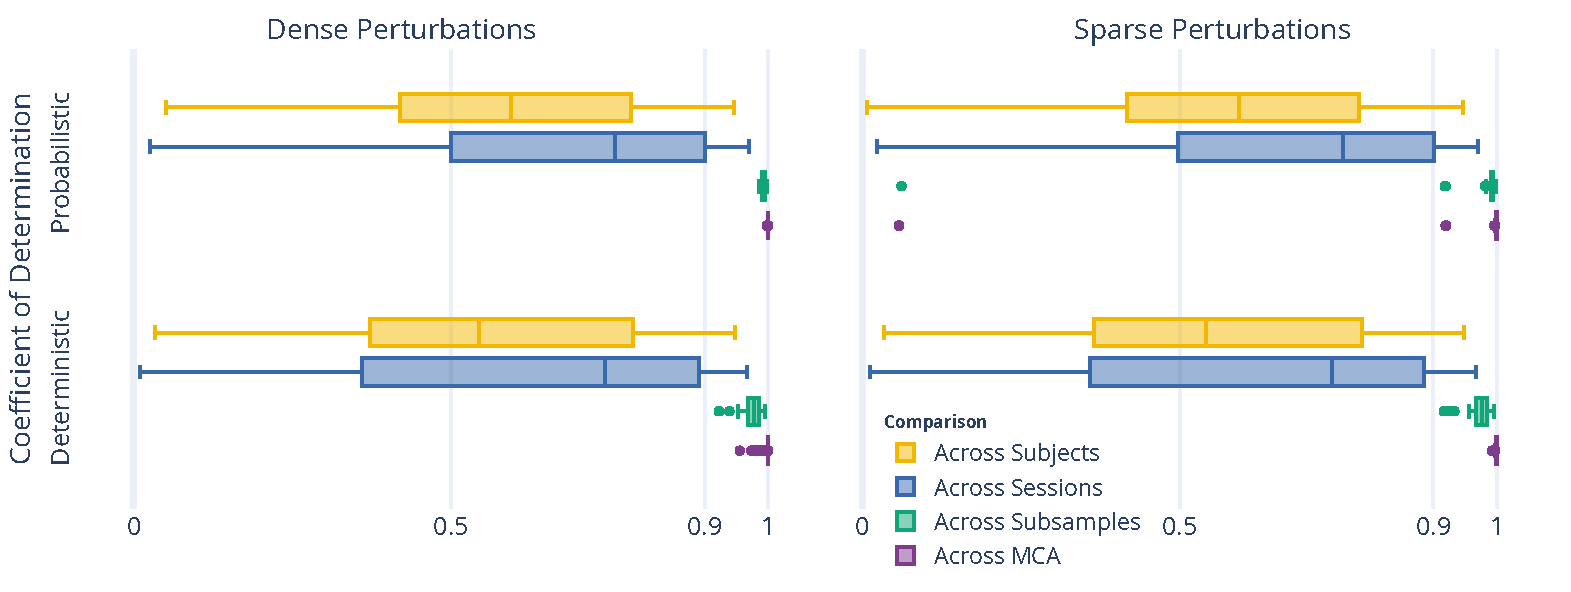
\includegraphics[width=\linewidth]{figures/figS1_correlation_differences.pdf}
\caption{The correlation between perturbed connectomes and their reference.}
\label{fig:correlation}
\end{figure}

\clearpage
\section{Complete Discriminability Analysis}
\label{supsec:discrimfull}

\begin{table*}[ht]\centering
\caption{The complete results from the Discriminability analysis, with results reported as mean~$\pm$~standard
deviation Discriminability. As was the case in the condensed table, the alternative hypothesis, indicating significant
separation across groups, was accepted for all experiments, with $p < 0.005$.}
\vspace{5pt}
% \fcolorbox{color1}{white}{%
% \parbox{\textwidth-2\fboxsep-2\fboxrule}{\centering
%   \colorbox{color2!10}{
%     \parbox{\textwidth-4\fboxsep-2\fboxrule}{

\begin{tabular}{llll|ll|ll|ll}
  &  &  &  &  \multicolumn{2}{l|}{\textbf{Reference Execution}} & \multicolumn{2}{l|}{\textbf{Dense Perturbations}} &  \multicolumn{2}{l}{\textbf{Sparse Perturbations}} \\
Exp. & Subj. & Sess. & Samp. & Det. &  Prob. &  Det. &    Prob. &     Det. &    Prob. \\
% Exp. & Subj. & Sess. & Dirs. & Sims. &     Discrim. (D) &    Discrim. (P) &     Discrim. (D) &    Discrim. (P) \\
\hline
1.1        &          All &      All &          1 & \cellcolor{color1!10}$ 0.64 \pm 0.00 $ & \cellcolor{color1!10}$ 0.65 \pm 0.00 $  & \cellcolor{color1!10}$ 0.82 \pm 0.00 $ & \cellcolor{color1!10}$ 0.82 \pm 0.00 $ & \cellcolor{color1!10}$ 0.77 \pm 0.00 $ & \cellcolor{color1!10}$ 0.75 \pm 0.00 $ \\
1.2        &          All &        1 &        All &  $ 1.00 \pm 0.00 $ &  $ 1.00 \pm 0.00 $ &  $ 1.00 \pm 0.00 $ &  $ 1.00 \pm 0.00 $ &  $ 0.93 \pm 0.02 $ &  $ 0.90 \pm 0.02 $ \\
1.3        &          All &        1 &          1 &        &  &  $ 1.00 \pm 0.00 $ &  $ 1.00 \pm 0.00 $ &  $ 0.94 \pm 0.02 $ &  $ 0.90 \pm 0.02 $ \\
& & & & & & & & & \vspace{-5pt}\\
2.4        &            1 &      All &        All &  \cellcolor{color1!10}$ 1.00 \pm 0.00 $ &  \cellcolor{color1!10}$ 1.00 \pm 0.00 $  &  \cellcolor{color1!10}$ 1.00 \pm 0.00 $ &  \cellcolor{color1!10}$ 1.00 \pm 0.00 $ &  \cellcolor{color1!10}$ 0.88 \pm 0.12 $ &  \cellcolor{color1!10}$ 0.85 \pm 0.12 $ \\
2.5        &            1 &      All &          1 &        &  &  $ 1.00 \pm 0.00 $ &  $ 1.00 \pm 0.00 $ &  $ 0.89 \pm 0.11 $ &  $ 0.84 \pm 0.12 $ \\
& & & & & & & & & \vspace{-5pt}\\
3.6        &            1 &        1 &        All &         &  &  \cellcolor{color1!10}$ 0.99 \pm 0.03 $ &  \cellcolor{color1!10}$ 1.00 \pm 0.00 $ &  \cellcolor{color1!10}$ 0.71 \pm 0.07 $ &  \cellcolor{color1!10}$ 0.61 \pm 0.05 $ \\
\end{tabular}


%     }
%   }
% }%
% }%

\label{stab:discrim_full}
\end{table*}

The complete discriminability analysis includes comparisons across more axes of variability than the condensed version.
The reduction in the main body was such that only axes which would be relevant for a typical analysis were presented.
Here, each of Hypothesis $1$, testing the difference across subjects, and $2$, testing the difference across sessions,
were accompanied with additional comparisons to those shown in the main body.

\paragraph{Subject Variation}
Alongside experiment $1.1$, that which mimicked a typical test-retest scenario, experiments $1.2$ and $1.3$ could be
considered a test-retest with a handicap, given a single aqcuisition per individual was compared either across
subsamples or simulations, respectively. For this reason, it is unsurprising that the dataset achieved considerably
higher discriminability scores. 

\paragraph{Session Variation}
Similar to subject variation, the session variation was also modelled across either both or a single subsample. In both
of these cases the performance was similar, and the finding that input perturbation reduced the off-target signal was
consistent.

\clearpage
\section{Univariate Graph Statistics}
\label{supsec:univar}

\begin{figure}[ht]\centering
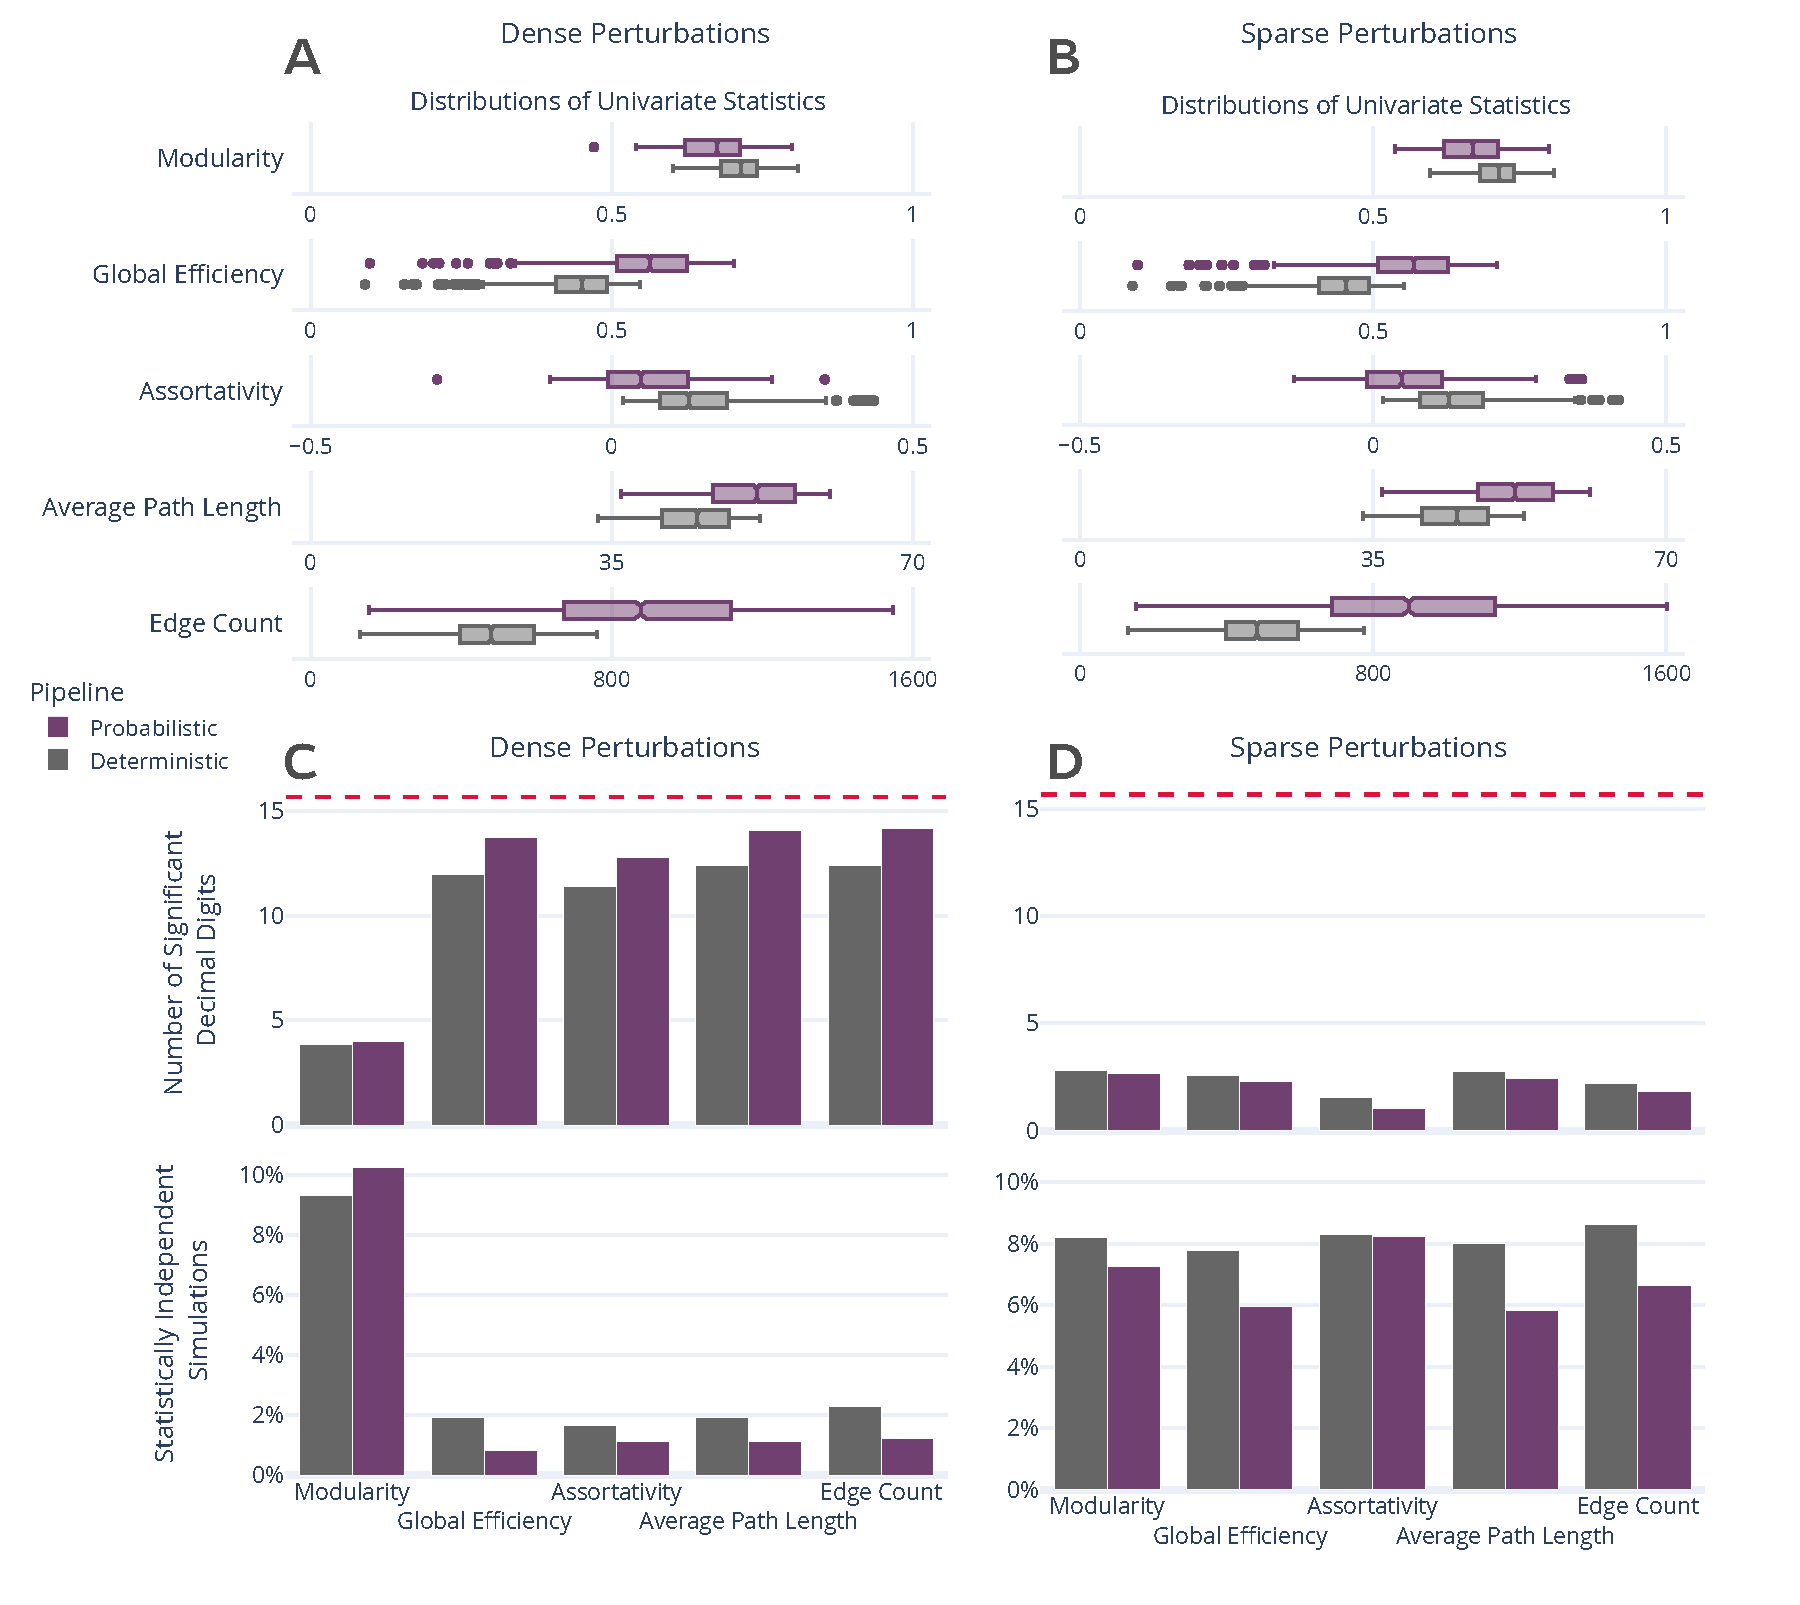
\includegraphics[width=\linewidth]{figures/figS2_univariate_differences.pdf}
\caption{Distribution and stability assessment of univariate graph statistics. (\textbf{A}, \textbf{B}) The
distributions of each computed univariate statistic across all subjects and perturbations for Pipeline and Input
settings, respectively. There was no significant difference between the distributions in A and B. (\textbf{C},
\textbf{D}; top) The number of significant decimal digits in each statistic across perturbations, averaged across
individuals. The dashed red line refers to the maximum possible number of significant digits.
(\textbf{C}, \textbf{D}; bottom) The percentage of connectomes which were deemed significantly different
($p < 0.05$) from the others obtained for an individual.}
\label{sfig:univariate}
\end{figure}

Figure~\ref{sfig:univariate} explores the stability of univariate graph-theoretical metrics computed from the perturbed
graphs, including modularity, global efficiency, assortativity, average path length, and edge count. When aggregated
across individuals and perturbations, the distributions of these statistics (Figures~\ref{sfig:univariate}A and
\ref{sfig:univariate}2B) showed no significant differences between perturbation methods for either deterministic or
probabilistic pipelines.

However, when quantifying the stability of these measures across connectomes derived from a single session of data, the
two perturbation methods show considerable differences. The number of significant digits in univariate statistics for
Pipeline Perturbation instrumented connectome generation exceeded $11$ digits for all measures except modularity, which
contained more than $4$ significant digits of information (Figure~\ref{sfig:univariate}C). When detecting outliers from
the distributions of observed statistics for a given session, the false positive rate (using a threshold of $p = 0.05$)
was approximately $2\%$ for all statistics with the exception of modularity which again was less stable with an
approximately $10\%$ false positive rate. The probabilistic pipeline is significantly more stable than the
deterministic pipeline ($p < 0.0001$; exploratory) for all features except modularity. When similarly evaluating these
features from connectomes generated in the input perturbation setting, no statistic was stable with more than $3$
significant digits or a false positive rate lower than nearly $6\%$ (Figure~\ref{sfig:univariate}D). The deterministic
pipeline was more stable than the probabilistic pipeline in this setting ($p < 0.0001$; exploratory).

Two notable differences between the two perturbation methods are, first, the uniformity in the stability of the
statistics, and second, the dramatic decline in stability of individual statistics in the input perturbation setting
despite the consistency in the overall distribution of values. It is unclear at present if the discrepancy between the
stability of modularity in the pipeline perturbation context versus the other statistics suggests the implementation of
this measure is the source of instability or if it is implicit to the measure itself. The dramatic decline in the
stability of features derived from input perturbed graphs despite no difference in their overall distribution both
shows that while individual estimates may be unstable the comparison between aggregates or groups may be considered
much more reliable; this finding is consistent with that presented for multivariate statistics.


\end{document}
